\documentclass{article}
\usepackage{graphicx}
\usepackage{longdivision}
\usepackage{enumitem}
\usepackage{amsmath}
\begin{document}
	\begin{titlepage}
		\centering
		\vfill
		\fbox{\Huge{Segunda práctica}} \\
		\vfill
		\large{\textsc{Hugo Tonatiuh Carrillo Bonilla}}\\
		\vfill
		320026379
		\vfill
		\begin{center}
			
\includegraphics[width=\linewidth]{./images/Portada.jpg}
		\end{center}
		\vfill
	\end{titlepage}

	\section*{Parte 1: Editor de texto.}
		\subsection*{Actividad 1.1}
		Yo utilizo el editor de texto Neovim. Lo utilizo por su simplicidad y gran capacidad. Lo utilizaré a lo largo de este curso por tres razones principales:
		\begin{itemize}
			\item Familiaridad: lo conozco desde hace años.
			\item Potencia: el lenguaje de programación de Java, al ser orientado a objetos, se beneficia ampliamente de las capacidades de procesamiento textual amplio de la familia de editores \texttt{vi}.
			\item Adaptabilidad: Existe un gran ambiente de extensiones y herramientas para Java.
			Además, es completamente gratis y de código abierto. Mientras que \textit{SublimeText} es de código cerrado y freemium.
			\begin{center}
				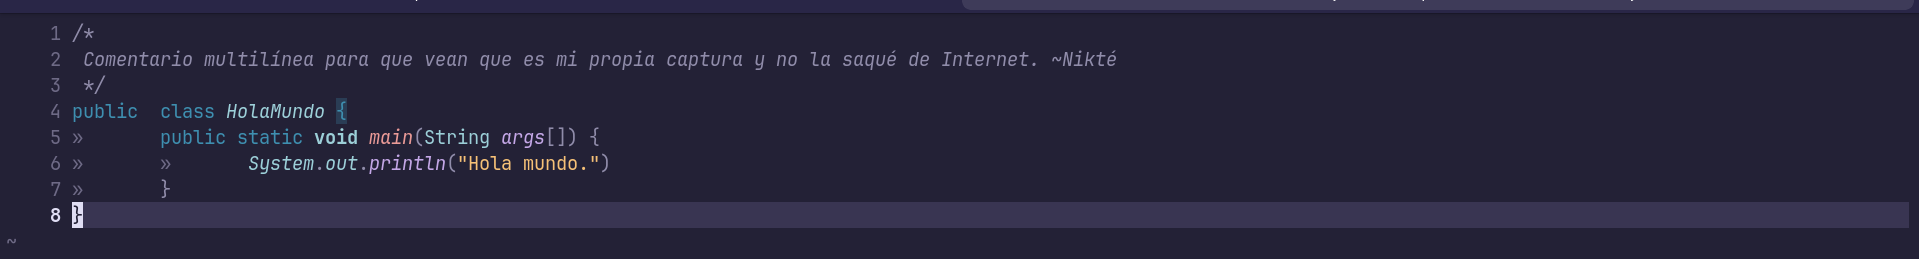
\includegraphics[width=\linewidth]{./images/P1-1.png}
			\end{center}
		\end{itemize}
		\subsection*{Actividad 1.2}
			\begin{enumerate}[label=\alph*]
				\item Pude abrir sin absolutamente ningún problema los archivos \texttt{.txt} y \texttt{.java}. \\
				Con los archivos \texttt{.docx} y \texttt{.xlsx} sucedió algo muy interesante: descubrí que \textit{Vim} tiene un plugin interno que te permite interactuar con archivos comprimidos y esto incluye a los xml. Entonces tuve acceso a un pseduomenú que después me permitía acceder individualmente a los archivos xml que estaban subcontenidos en cada archivo propietario de Windows.
					\begin{center}
						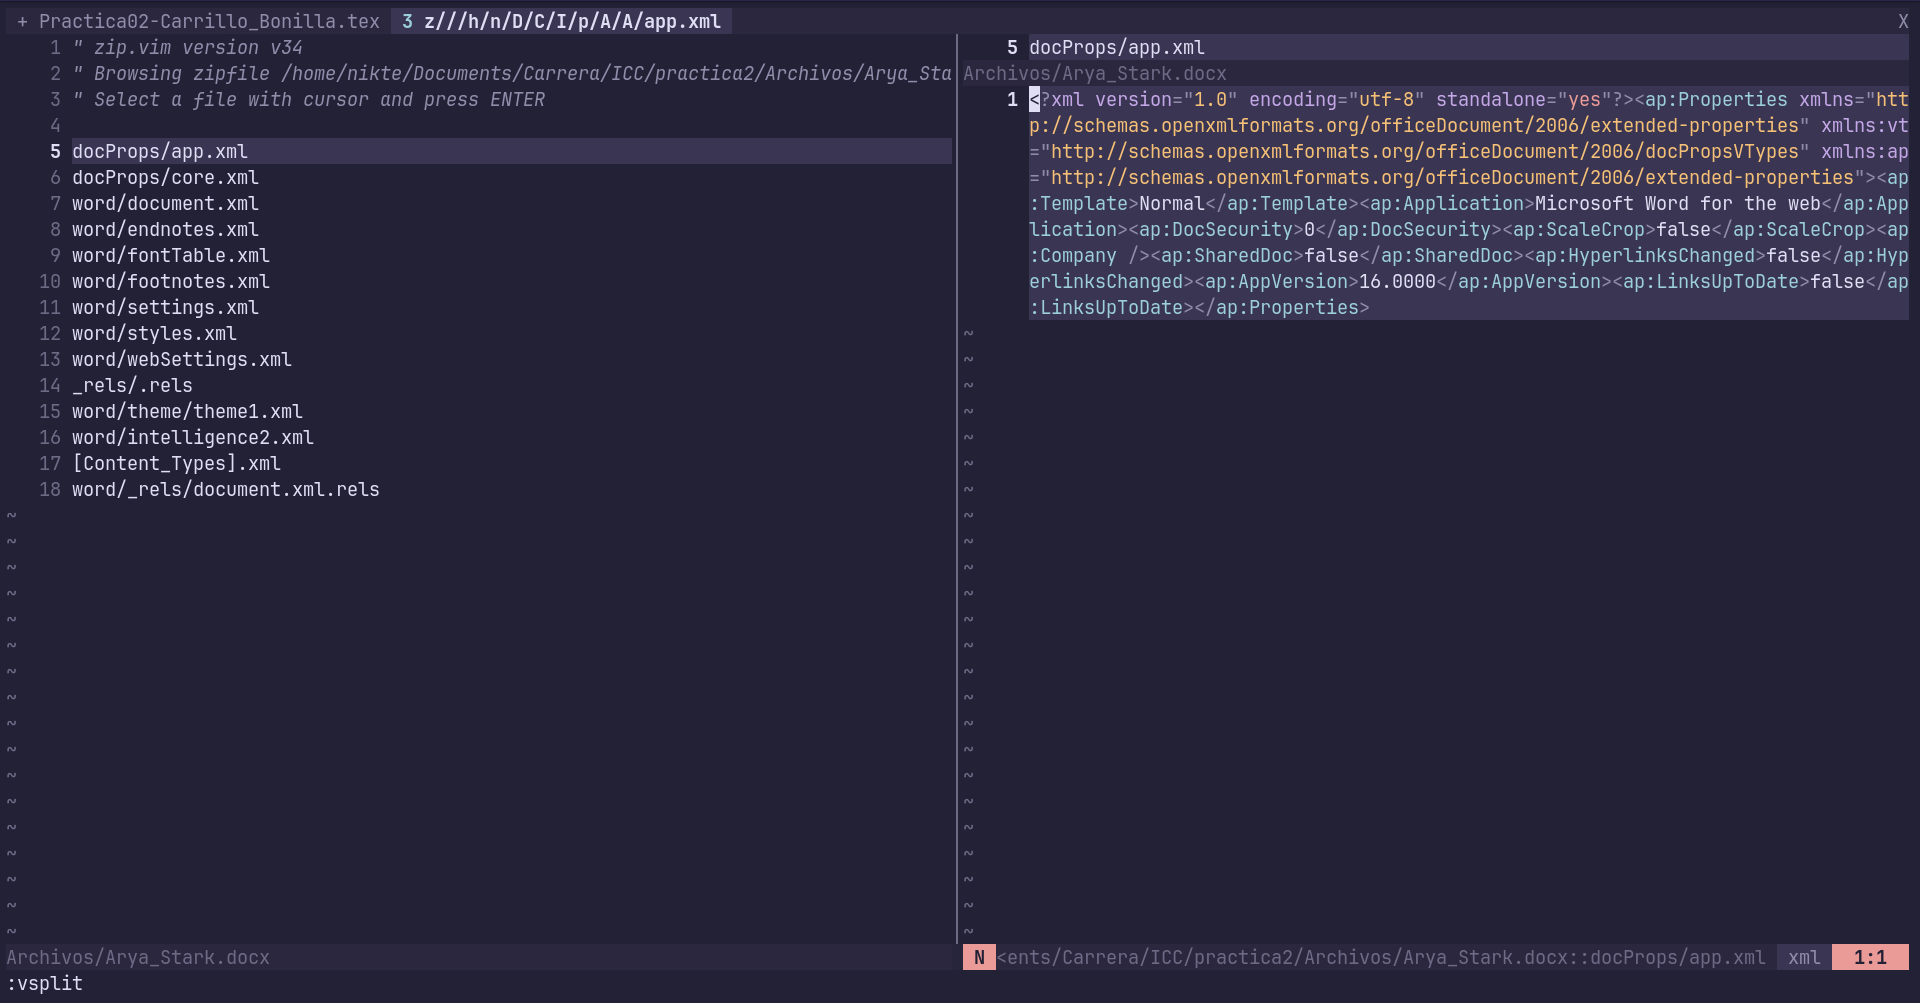
\includegraphics[width=\linewidth]{./images/P1-2-1.png}
					\end{center}
					Finalmente, con los archivos \texttt{.pdf} y \texttt{.png} solo ví un montón de caracteres aleatorios sin ton ni son.
				\item La razón por la que puedo abrir perfectamente los archivos de texto y de Java es precisamente porque son archivos de texto pensados para ser mostrados en un editor de texto plano, los archivos propietarios de Windows en realidad son empaquetadores elegantes para muchos archivos del tipo xml. Finalmente, los archivos de \texttt{.pdf} y \texttt{.png} son archivos principalmente visuales que codifican su información a través de ecuaciones o mapas.
			\end{enumerate}
	\section*{Parte 2: JShell}
		\subsection*{Actividad 2.1}
			\begin{center}
				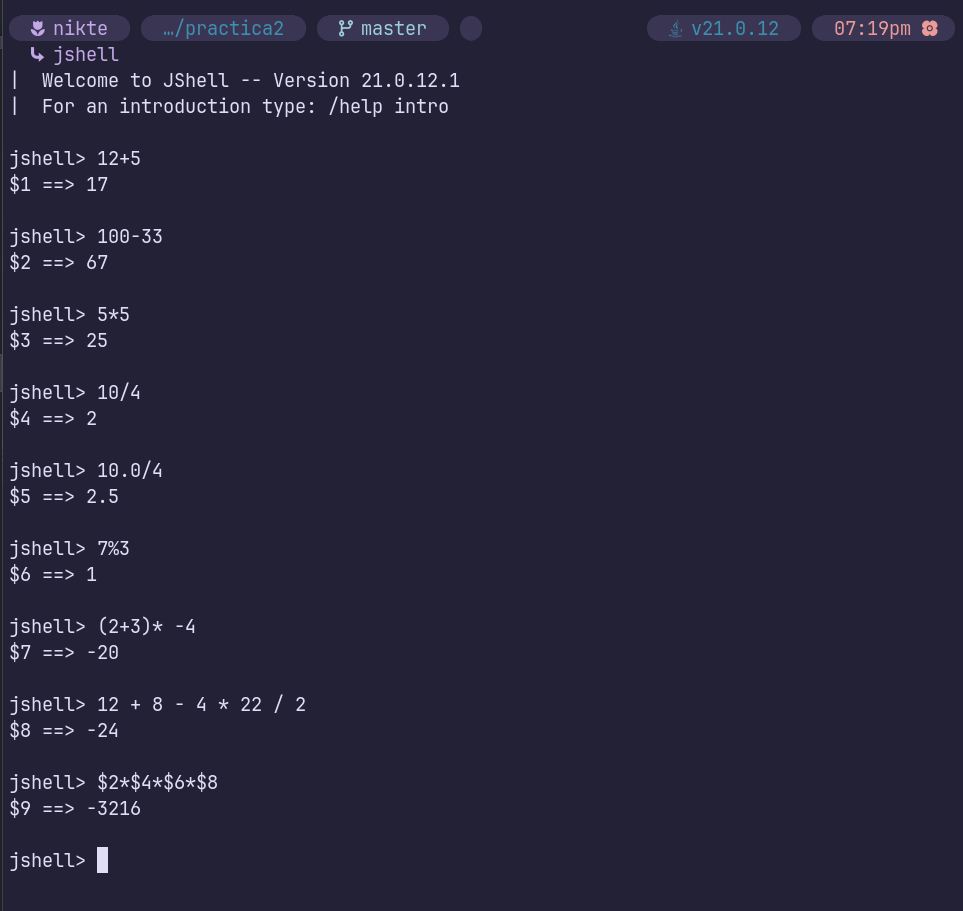
\includegraphics[width=\linewidth]{./images/P2-1-1.png}
			\end{center}
			Mi laptop soñada es la \textit{Lenovo ThinkPad P16s} sus características son:
			\begin{itemize}
				\item Procesador Intel i9
				\item 32 GB de RAM
				\item 1 TB de memoria SSD
			\end{itemize}
			Para calcular su precio sin IVA, guardé su precio en total en una variable, guardé la diferencia entre el 100\% y el porcentaje sin IVA en otra variable, y realicé la siguiente operación con estas dos variables: $$ \text{Precio}\cdot\text{Diferencia}\times 10^{-2} $$.
			\begin{center}
				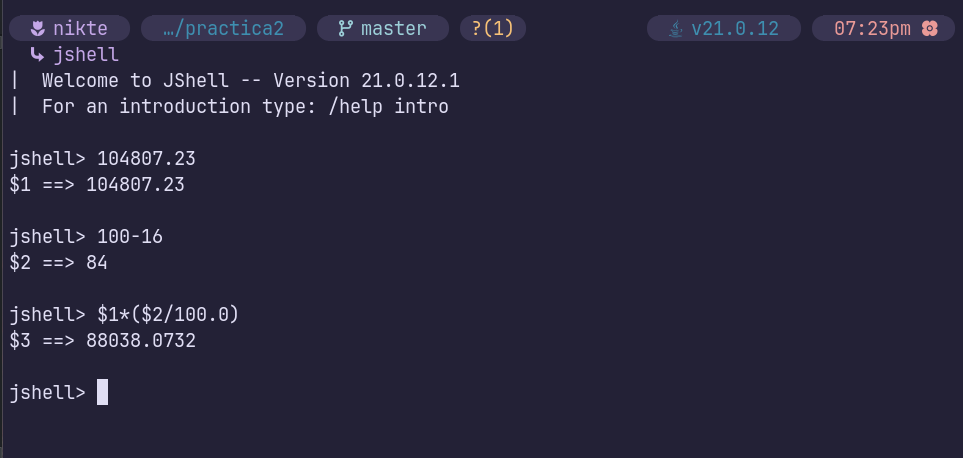
\includegraphics[width=\linewidth]{./images/P2-1-2.png}
			\end{center}
		\subsection*{Actividad 2.2}
			\begin{center}
				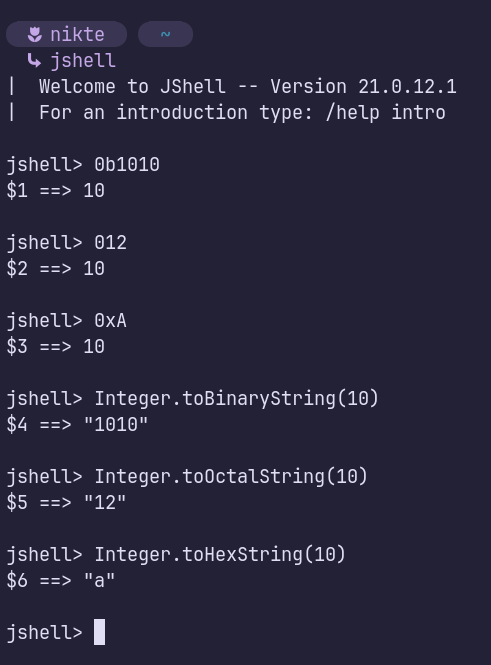
\includegraphics[width=\linewidth]{./images/P2-2-1.png}
			\end{center}
			\newpage
			\subsubsection*{Decimal a binario.}
				\begin{enumerate}
					\item \intlongdivision{13}{2} \intlongdivision{6}{2} \intlongdivision{3}{2} \intlongdivision{1}{2}
					\item \intlongdivision{42}{2} \intlongdivision{21}{2} \intlongdivision{10}{2} \intlongdivision{5}{2} \intlongdivision{2}{2} \intlongdivision{1}{2}
				\end{enumerate}
			\subsubsection*{Binario a decimal.}
				\begin{enumerate}
					\item $$ 1001001_2 = (1 \cdot 2^0) + (0 \cdot 2^1) + (0 \cdot 2^2) + (1 \cdot 2^3) + (0 \cdot 2^4) + (0 \cdot 2^5) + (1 \cdot 2^6) = 73_{10} $$
					\item $$ 11011011_2 = (1 \cdot 2^0) + (1 \cdot 2^1) + (0 \cdot 2^2) + (1 \cdot 2^3) + (1 \cdot 2^4) + (0 \cdot 2^5) + (1 \cdot 2^6) + (1 \cdot 2^7)= 219_{10} $$
				\end{enumerate}
				\begin{center}
					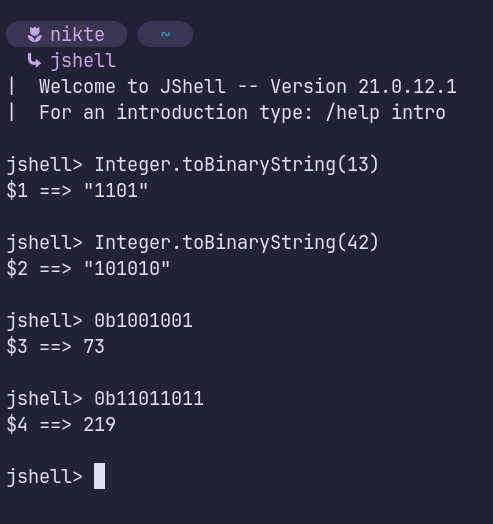
\includegraphics[width=\linewidth]{./images/P2-2-2.png}
				\end{center}
	\section*{Parte 3: Autopsia de un programa}
		\subsection*{Actividad 3.1}
			Así me corrió el Hola Mundo:
			\begin{center}
				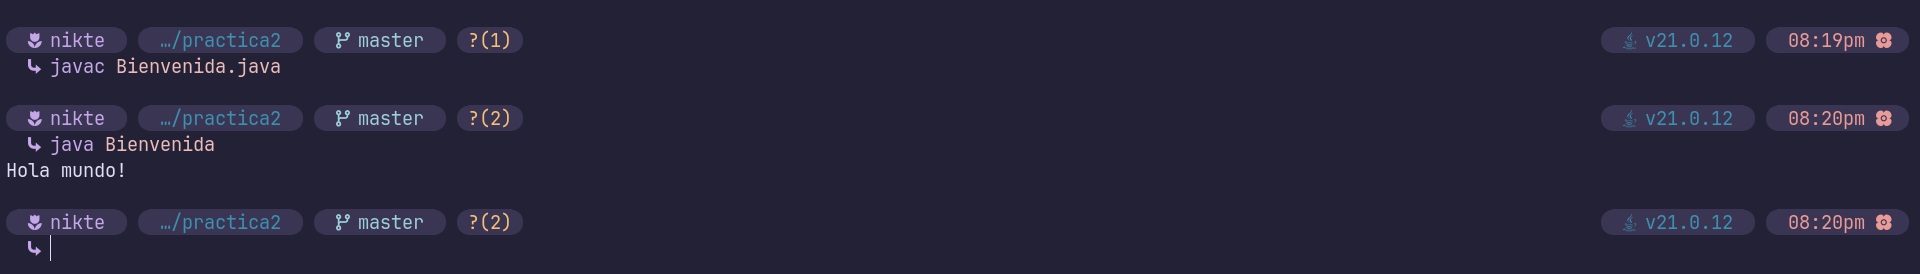
\includegraphics[width=\linewidth]{./images/HolaMundo.png}
			\end{center}
			Para el ejercicio 4 modifiqué así el programa:
			\begin{center}
				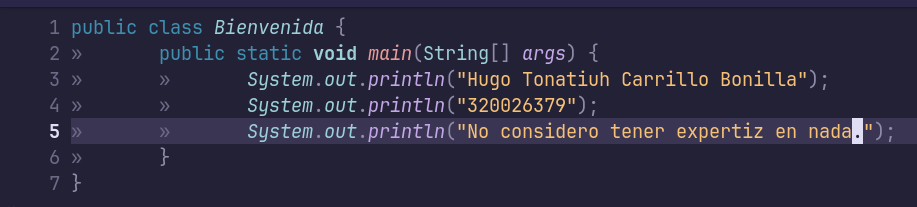
\includegraphics[width=\linewidth]{./images/P3-1-1.png}
			\end{center}
			Mientras que para el ejercicio 5 lo modifiqué así:
			\begin{center}
				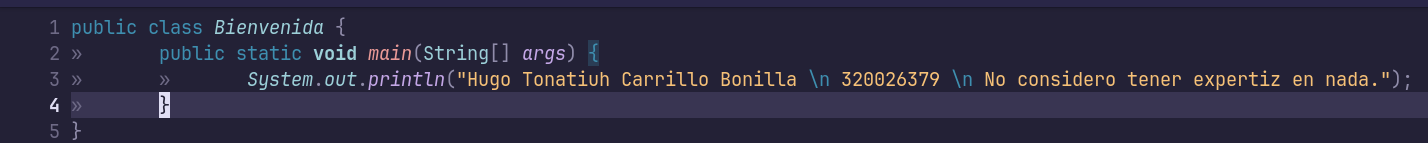
\includegraphics[width=\linewidth]{./images/P3-1-2.png}
			\end{center}
			Compiló así:
			\begin{center}
				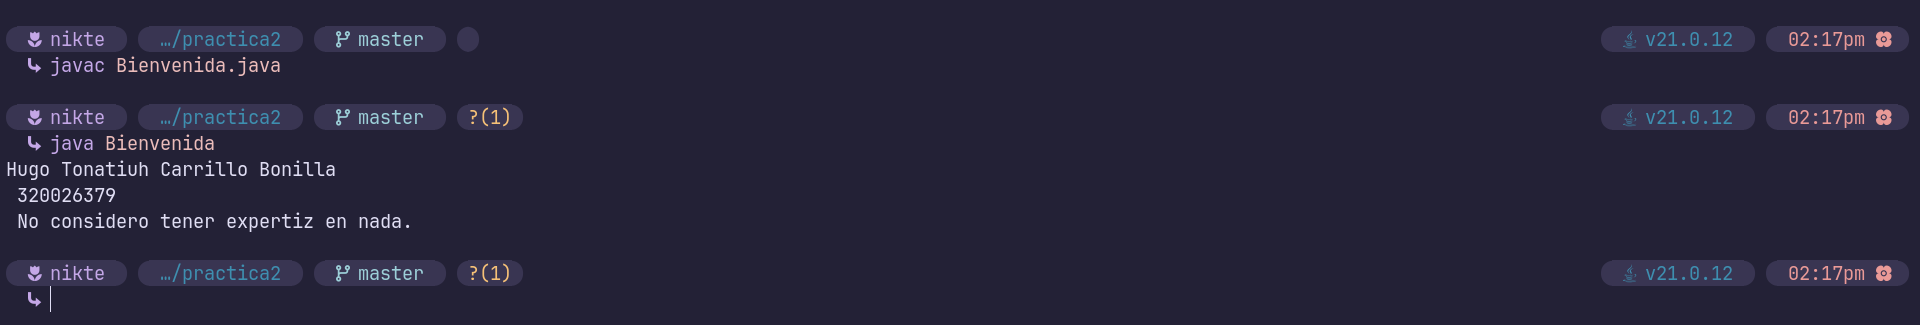
\includegraphics[width=\linewidth]{./images/P3-1-3.png}
			\end{center}
		\subsection*{Actividad 3.2}
			Los errores que se encontraron al principio fueron:
			\begin{enumerate}
				\item Línea 5. Código mal escrito. Faltaba cerrar un paréntesis. \texttt{Errores.java:5: error: ')' or ',' expected}. Se corrige añadiendo el paréntesis final \textbf{antes} del punto y coma.
				\item Línea 6. Código mal escrito. Faltaba cerrar una string. \texttt{Errores.java:6: error: unclosed string literal}. Se corrige añadiendo las comillas finales.
				\item Línea 12. Código mal escrito. No se termina adecuadamente una expresión. \texttt{Errores.java:12: error: ';' expected}. Se corrige añadiendo punto y coma al final.
				\item Línea 7. Código sin sentido. El compilador piensa que queremos restar strings. \texttt{Errores.java:7: error: bad operand types for binary operator '-'}. Ponemos la resta entre paréntesis.
				\item Línea 10. Código sin sentido. Le dimos una string a una función que solo acepta enteros. \texttt{Errores.java:10: error: incompatible types: String cannot be converted to int}. Le quitamos las comillas al argumento dentro de la función.
				\item Línea 8. Código con resultado incorrecto. Dividimos dos enteros pero queremos un float. No arroja errores porque hace lo que le pedimos, no supimos expresar lo que queríamos. Cambiamos alguno de los valores divididos a un float.
				\item Línea 9. Código con resultado incorrecto. Nuestro orden de operaciones es incorrecta. No arroja errores porque hace lo que le pedimos, no supimos expresar lo que queríamos. Insertamos paréntesis para que el orden de operaciones sea explícito.
				\item Línea 11. Código con resultado incorrecto. Exigimos que la función \texttt{Integer.parseInt} nos devuelva un número en base 8, pero queremos que nos devuelva 39, y para eso necesitamos que traduzca un número en base 5. No arroja errores porque hace lo que le pedimos, no supimos expresar lo que queríamos. Cambiamos el segundo argumento de la función por 5.
			\end{enumerate}
			\begin{center}
				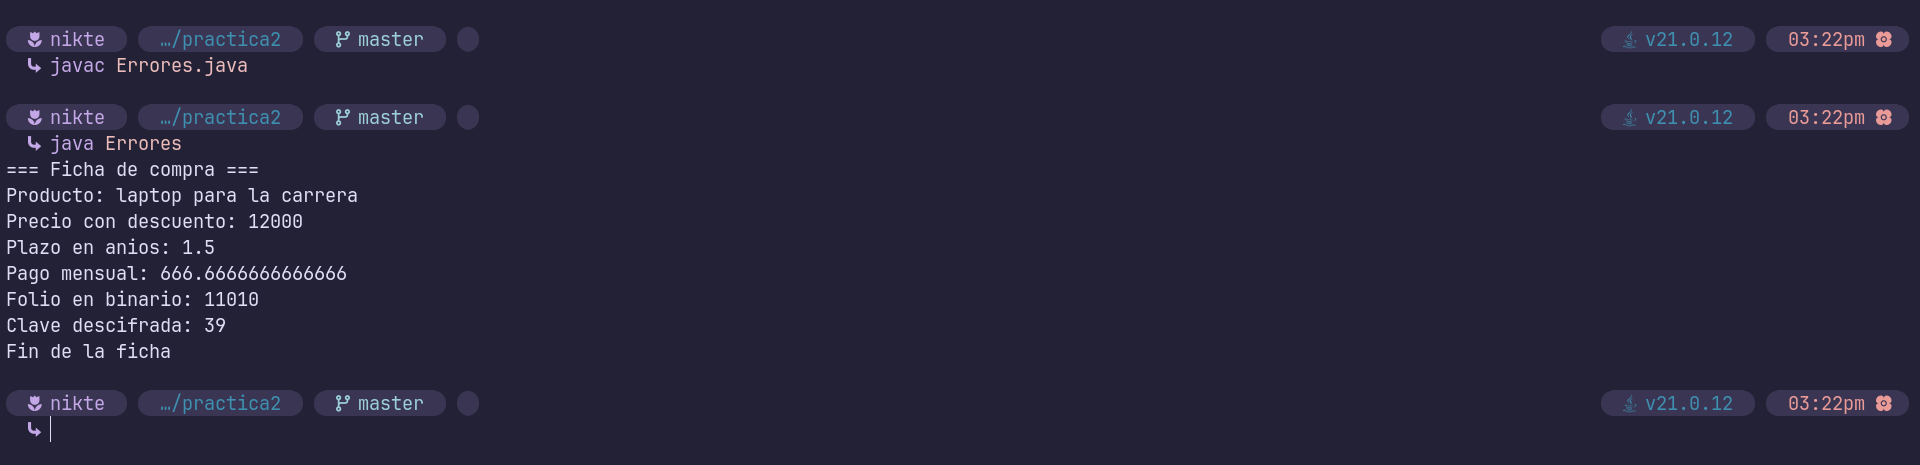
\includegraphics[width=\linewidth]{./images/P3-2-1.png}
			\end{center}
	\section*{Conclusión}
		En esta práctica me familiaricé con los errores y logs del compilador de Java. Me salió un error que no me pareció prudente comentar pero es apropiado señalar aquí: la \textit{Java Virtual Machine} es muy sensible con que le demos la clase correcta, y para eso nos debemos de encontrar en el mismo directorio en el que se encuentra nuestro archivo \texttt{.class}. Eso me pareció interesante, y gracias a este error aprendí un poco sobre cómo la JVM corre e inicializa los programas compilados. Escuché por primera vez los términos \texttt{ClassLoader}, \texttt{ObjectLoader}, \texttt{ClassPath}, \textit{JAR Hell} entre otros. Estos son conceptos por los que me emociona mucho empezar a aprender.
\end{document}
